\chapter{Appendix}
\label{chap:appendix}

A few experiments / results that are not that relevant for the scope of this thesis are mentioned in this section.

\section{Sampler parallelization}
\label{sec:sampler_parallelization}
Figure \ref{fig:sampler_parallelization} shows the benchmark results between the naive sampler with and without parallelization.
The benchmark was performed on a singular NVIDIA Ampere A100 GPU.
\begin{figure}[h]
    \centering
    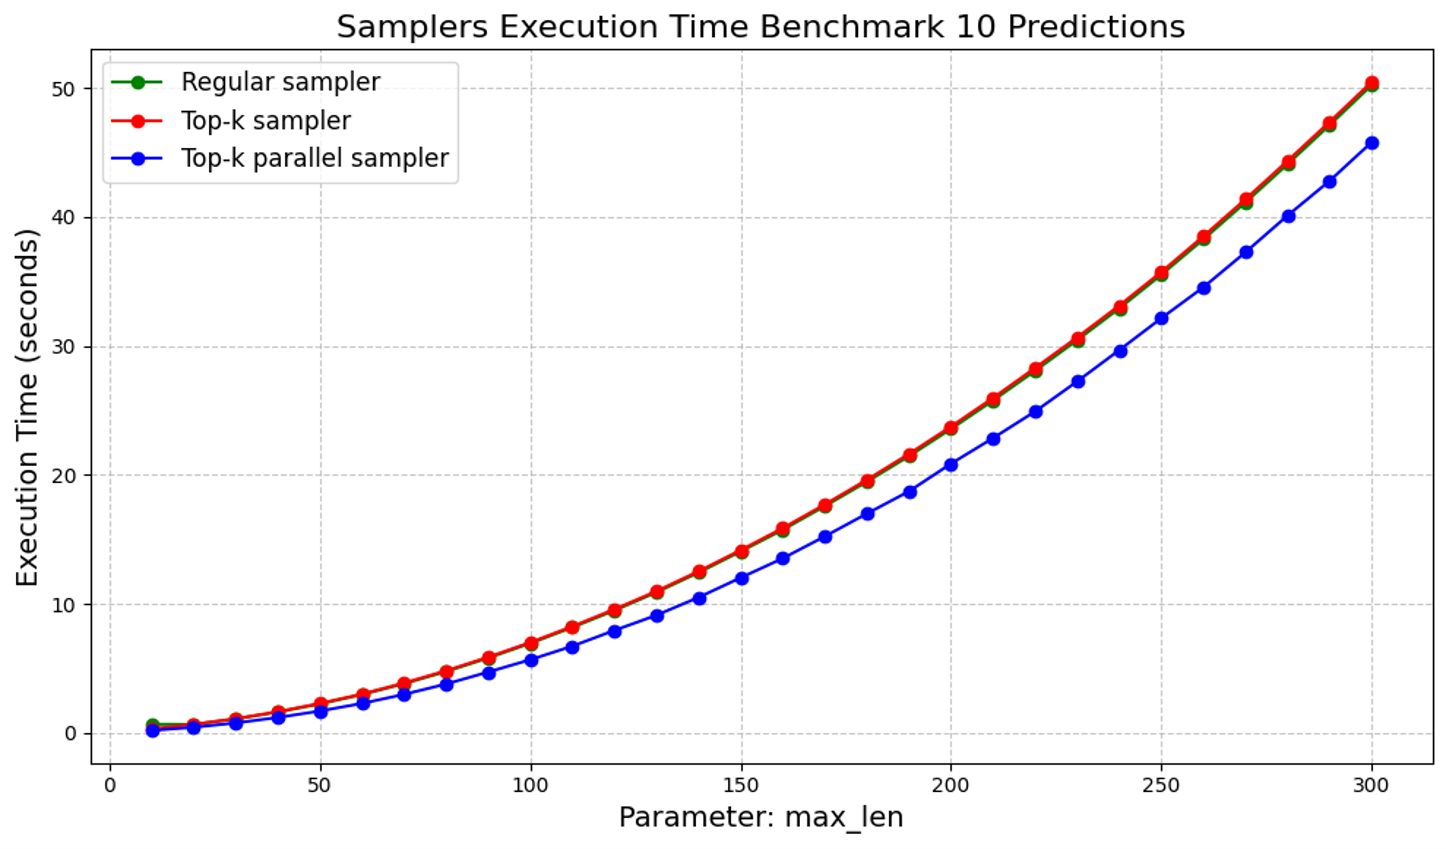
\includegraphics[width=0.6\linewidth]{figures/appendix/sampler_parallel.png}
    \caption{Execution Time Benchmark sampler parallelization}
    \label{fig:sampler_parallelization}
\end{figure}

The naive sampler shows to be more computationally efficient with parallelization.
A small difference in execution time can be substantial when this sampler is called thousands of times.
All further stochastic samplers in this thesis were executed with this parallelization enabled.

\section{Stochastic samplers benchmark full results}
\label{sec:sampler_full_results}

Figures \ref{fig:top-k_appendix}, \ref{fig:top-k_zoomed_appendix}, \ref{fig:top-p_appendix}, \ref{fig:top-p_zoomed_appendix} show the full results from the top-k and top-p benchmark.

\begin{figure}[h]
    \centering
    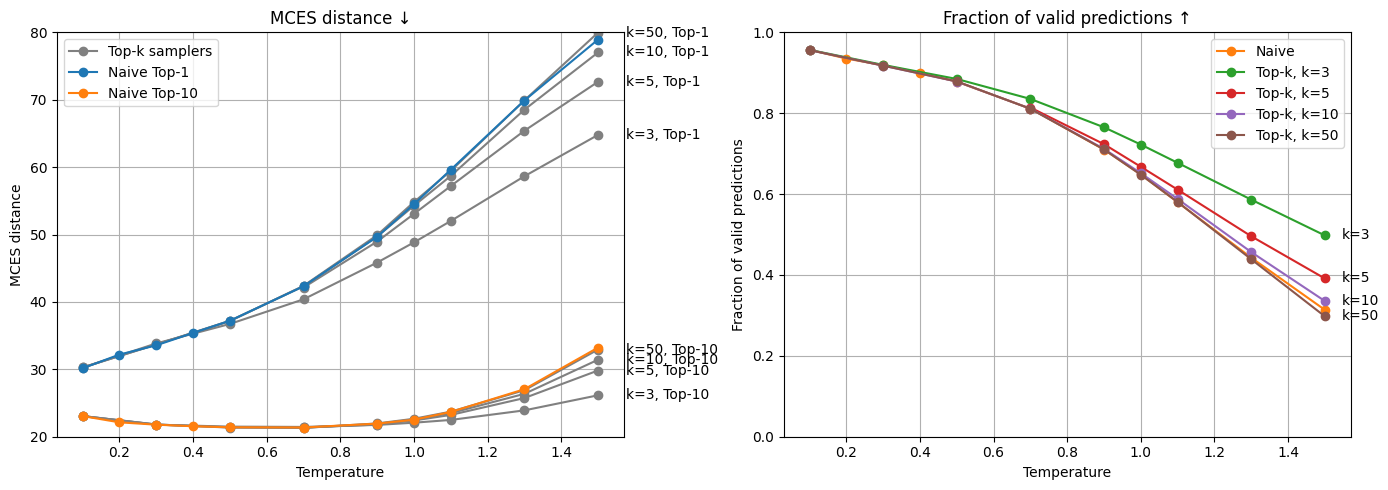
\includegraphics[width=\linewidth]{figures/appendix/samplers/top-k_vs_naive.png}
    \caption{Full top-k benchmark with top-1 and temperature search results}
    \label{fig:top-k_appendix}
\end{figure}

Top-k with $k=20$ is left out of figure \ref{fig:top-k_appendix} for readability. These results are in line with the others.

\begin{figure}[h]
    \centering
    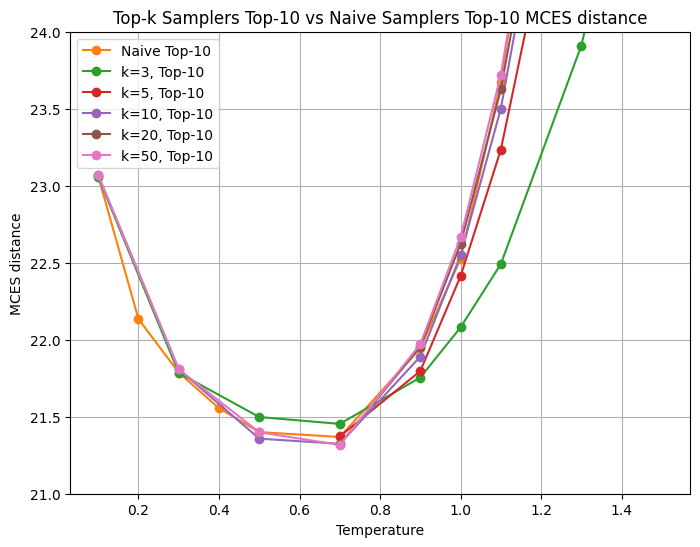
\includegraphics[width=0.6\linewidth]{figures/appendix/samplers/top-k_vs_naive_top-10.png}
    \caption{Zoomed in top-k top-10 MCES distance}
    \label{fig:top-k_zoomed_appendix}
\end{figure}

Figure \ref{fig:top-k_zoomed_appendix} shows the slight improvement of top-k $k\geq 10$ to the naive sampler in the temperature optima.

\begin{figure}[h]
    \centering
    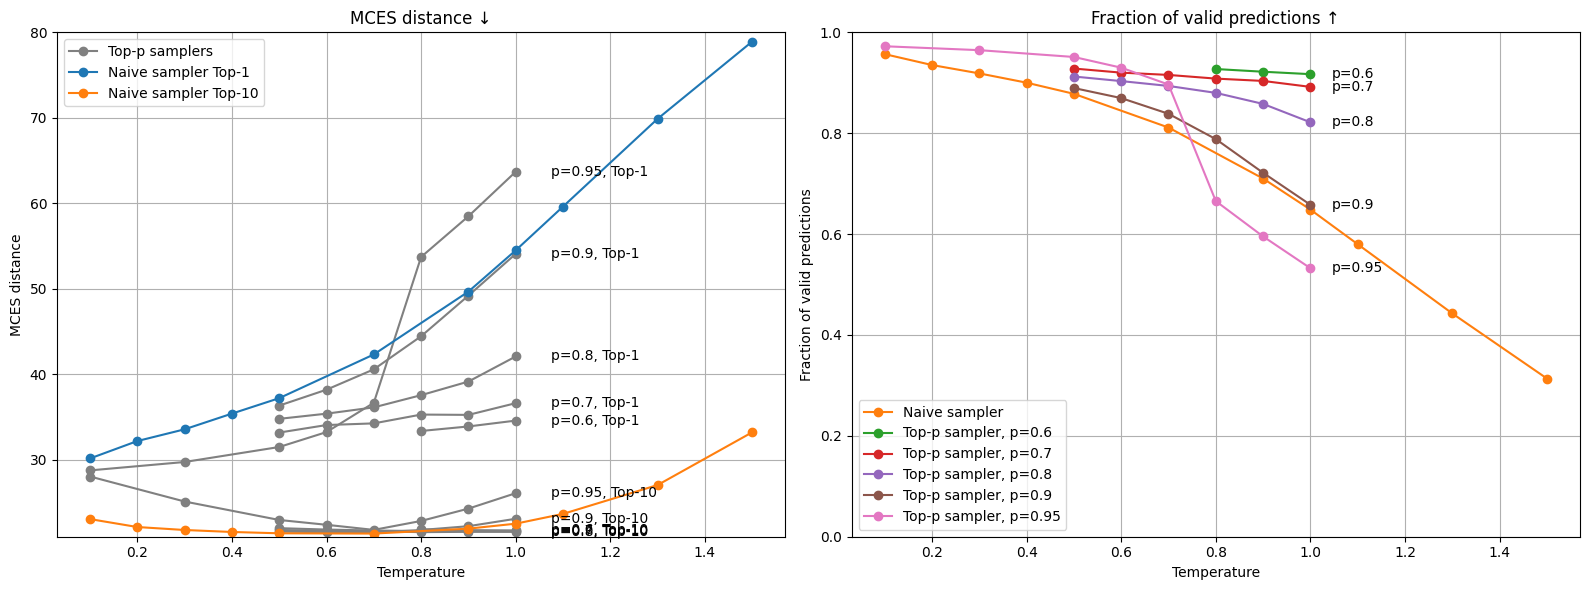
\includegraphics[width=\linewidth]{figures/appendix/samplers/top-p_vs_naive.png}
    \caption{Full top-p benchmark with top-1 and temperature search results}
    \label{fig:top-p_appendix}
\end{figure}

The search grid for the top-p benchmark was for some values of $p$ cut short to save resources.

\begin{figure}[h]
    \centering
    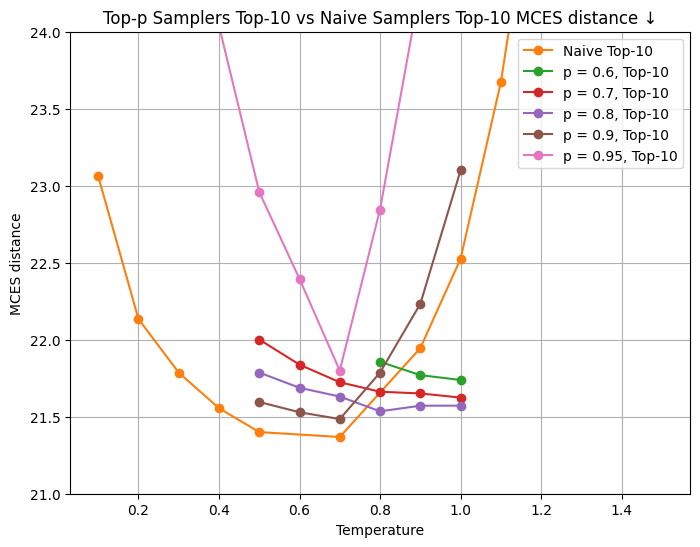
\includegraphics[width=0.6\linewidth]{figures/appendix/samplers/top-p_vs_naive_top-10.png}
    \caption{Zoomed in top-p top-10 MCES distance}
    \label{fig:top-p_zoomed_appendix}
\end{figure}

Figure \ref{fig:top-p_zoomed_appendix} shows that the top-p sampler results do not exceed the results from the naive sampler in their temperature optima.


\section{BPE benchmark full results}
\label{sec:bpe_appendix}

\begin{figure}[h]
    \centering
    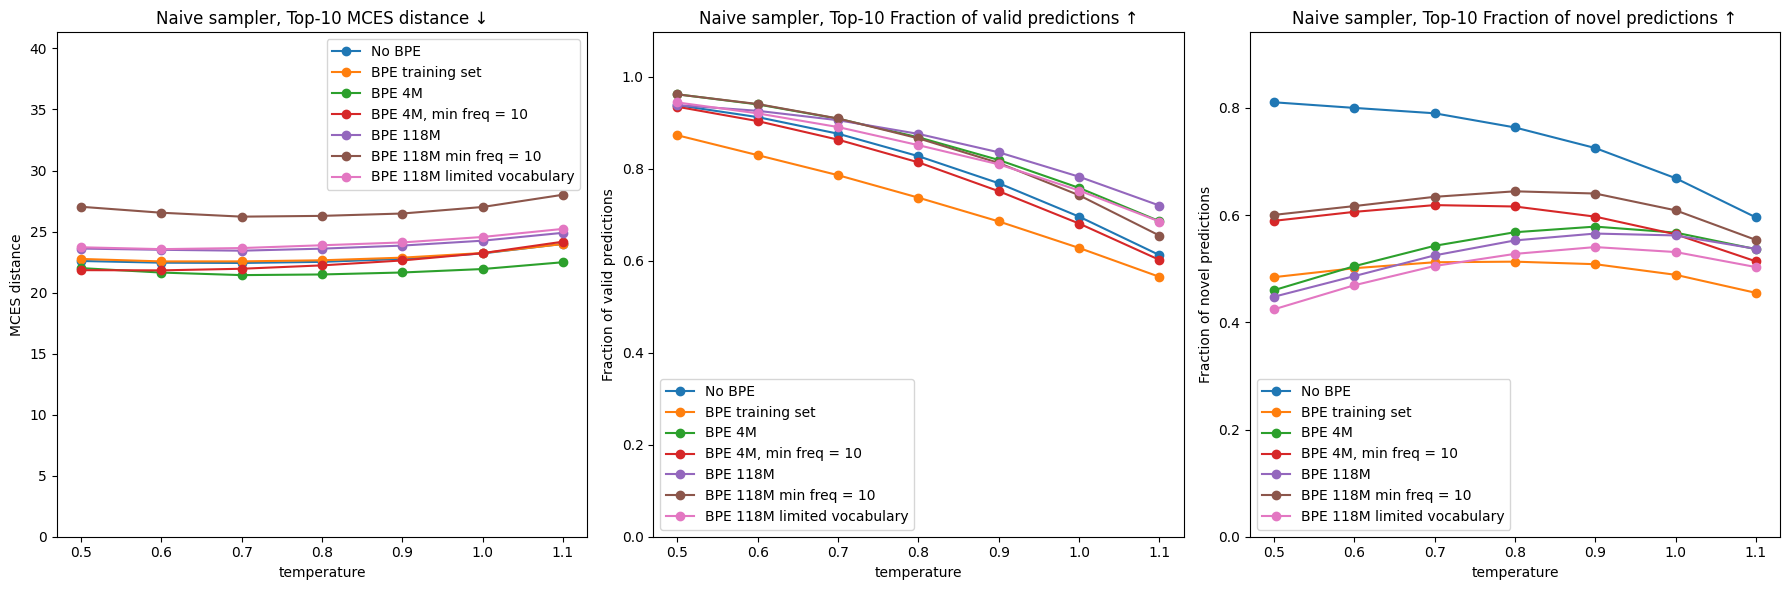
\includegraphics[width=1.0\textwidth]{figures/appendix/bpe.png}
    \caption{Full BPE experiment results}
    \label{fig:bpe_appendix}
\end{figure}